
    
%%%%%%%%%%%%%%%%%%%%%%%%%%%%%%%%%%%%
\chapter{Literature Review} 
\label{chap:Literature_Review}
This section covers the baseline (section \ref{sec:handcrafted}) and state of the art models (section \ref{SoTA})  used within IAQA literature makes a definition of the data used and reviews various Hand-Crafted (HC) as well as deep learning approaches to IAQA. Within deep learning we also include (Vision Transformers) ViTs and (Convolutional Vision Transformers) ConVits  and examine different attention mechanism used in DNNs (section \ref{sec:attention machanisms}). In (section \ref{sec:a case for dl})  we make a case for deep learning over HC feature extraction and the reason for using the Aesthetic Visual Analysis (AVA) benchmarking dataset. We do this through conducting systematic review of datasets and conducting meta analysis of literature through the \textit{`lense'} of datasets used in IAQA literature and descriptive as well as parametric analysis of the AVA dataset meta data (section \ref{sec:related_data}). Finally we outline the evaluation metrics used for IAQA as a binary classification problem in section \ref{sec:evaluation_metrics}. 


%%%%%%%%%%%%%%%%%%%%%%%%%%%%%%%%%%%%
\section{Related Work (Image Aesthetic Quality Assessment)}
\label{related_work}


Image Aesthetic Quality Assessment (IAQA)\footnote{Within the literature on image quality, some publications - which are clearly within the domain of IAQA - refer to this simply as Quality Assessment (QA)\cite{Chang2017}; others heavily blur these categories\cite{Kanwal2021}. For disambiguation, here it is referred to as IAQA so as to delineate the field from other domains - such as image restoration - clearly.} is a highly nuanced and challenging area, which requires care and consideration at several layers of detail. 

\par At a high level within the literature on IAQA, there has been a shift from HC to deep features, in addition to the consideration of either visual attention mechanisms or model architectures. This is reflective of the wider trend in computer vision. Further to what is outlined in the introduction, here we narrow the focus to intra-IAQA literature, rather than interrelated sub-fields or domains that focus on painting or calligraphy\cite{Fernando2021,Sun2015} etc.

There are, to date, four reviews (experimental and literature) on IAQA\cite{Yang2019, Kanwal2021, Deng2017,Spathis2016}. These provide an initial high-level view into IAQA, and cover approaches both HC and many - but not all - of the datasets used in IAQA research publications. The prevalence of citation and review of various IAQA datasets is shown in the Venn diagram (figure \ref{fig:venn}). 


\subsection{Baseline}
\label{sec:baseline}

Initial approaches taken to HC features Trainee Classifier on Support Vector Machines (SVM) or Gaussian Mixture Models: Here, we consider approaches that have used deep learning, alongside performance within IAQA rather than classification more widely.

Deep learning models have generally been binary classification, where MOS is thresholded $<5=0$ and $>5=1$ to produce binary ground truth  of $\in \{0,1\} = \in \{bad,good\}$ image quality. 

As has already been outlined, some form of attention mechanism, paralleling, or patching has been used to improve results on various vanilla CNNs that have been used for IAQA as an image classification problem:\begin{description}
    \item[Alexnet]\cite{Krizhevsky2017a} by \cite{Koa2016b};
    \item[VGG16]\cite{Simonyan2015a} by \cite{Ma2017,Deng2017, Mai2016, Hosu2019, Sheng2018,Ma2017,Kong2016,Liu2017,Koa2016b};
    \item[Inception Nets]\cite{Szegedy2016} by \cite{Liu2020a,Talebi2018};
    \item[GoogleNet]\cite{Szegedy2015} by \cite{Jin2019,Hii2017a};
    \item[DenseNet]\cite{Huang2017} by \cite{Liu2020,Liu2020a};
    \item [MobileNet]\cite{Howard2017} by \cite{Talebi2018};
    \item [ResNets]\cite{He2016a} $\in \{18,34,50,101,152\}$ by  \cite{Sheng2018,Kong2016,Koa2016b,She_2021_CVPR,Chen2020b,Liu2020a}. 
\end{description}  

These report an overall accuracy of VGG with AVA zero padded to square of 72.9\%\cite{Ma2017}, which is significantly less than the performance of ResNet152, reproduced here at 74.1\%. Further, when comparing hybrid vision transformers \textit{ConViTs}, many publications take ResNet architecture as baseline\cite{Wu2021,El-Nouby2021a,Khan2021}, with more recent publications using ResNet152\cite{Jin2019}. Here, training ResNet $\in \{18,50,152\}$ to produce baseline metrics. 

Figure \ref{fig:resnet_block} shows one residual block, of which 18 make up the smaller ResNet figure \ref{fig:resnet_compared}. These networks perform well, and are arguably more competitively efficient with fewer floating point operations (FLOPS). Each block has two weight layers, allowing for an $x$ or identity layer to be concatenated back (a technique for countering vanishing gradients/keeping residual values). All of these networks are trained as baselines without attention mechanisms, but do not require consideration as far as feature hierarchy as this is a built in feature of CNNs\cite{He2016} . Generally within IAQA, where an architecture is used to provide baseline metric, it is also used within a model as a backbone - although, this is not always the case. Authors have taken various approaches to copping, such as canter copping or warping to dimension $ 3 \times 224 \times 224$.  

\begin{equation}
    y = f(x\{W_i\})+x
\end{equation}

Where the output of one residual block x is input $W_i$ are weights of $i_th$ layer in the residual block. 

\begin{figure}
    \centering
    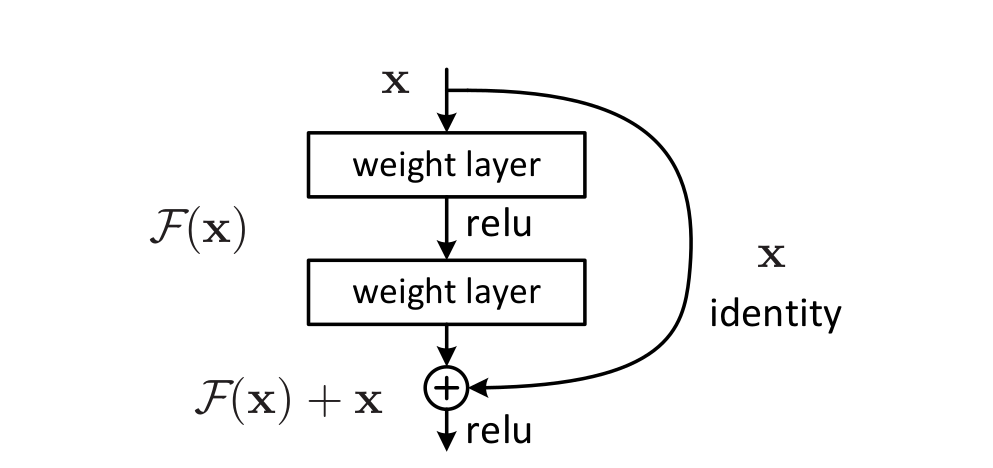
\includegraphics[width=0.38\textwidth]{figures/Literature Review/resnetblock.png}
    \caption{ResNet Block \cite{He2016}}
    \label{fig:resnet_block}
\end{figure}

\begin{figure}
    \centering
    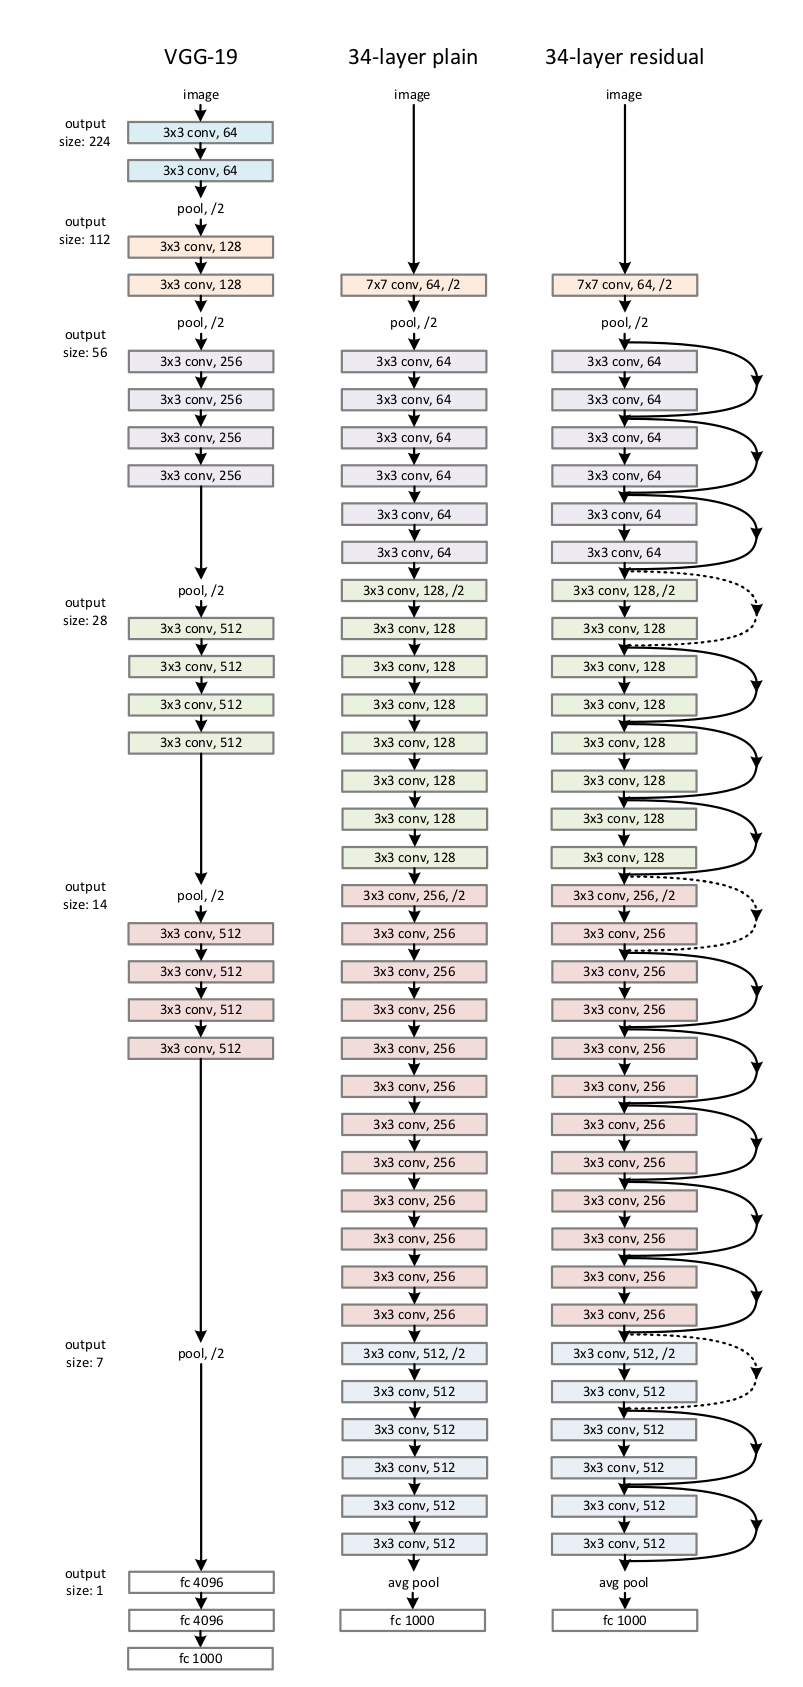
\includegraphics[width=0.3\textwidth]{figures/Literature Review/resnet.png}
    \caption{VGG-19 left , 34 Layer plain middle, ResNet 18 (19 blocks) right  \cite{He2016a}  }
    \label{fig:resnet_compared}
\end{figure}
%%%produced with resent 152,18' 

\subsection{Digital Images}


All of the IAQA techniques reviewed are, by necessity, digital images produced using the sensor arrays of commercially available digital cameras (whose sensors are sensitive to light within an extremely narrow section of the electromagnetic spectrum of $0.4 \times 10^{-4} $ (violet) and $0.7 \times 10^{-6}$ (red)) and digital images discrete quantized representations 0-255 or $0 < (2^{8})-1$ of this spectrum. 

Colour digital images are captured as three channels in an \textit{RGB} image; traditional technique applies functions across an image array $f(x,y)$ where $x$ and $y$ are spatial coordinates of a pixel array. 

\subsection{State of the Art (SoTA)}
\label{SoTA}

Three main and closely interrelated features exist for deep learning based models, \textit{multi column}, \textit{patching of image}, and \textit{attention}. For clarity and focus, here we evaluate models that are compared on the AVA benchmark dataset, as it has become the convention within IAQA to benchmark on AVA dataset. 


\subsubsection{Multi Column} 

 Almost all models have used some form of multi column image classification network as a backbone; the performance accuracy of each is shown in \ref{tab:SOA}. 
 
 Even where the multi patch is not apparent in name, this is embedded in the approach in some way. Early models, such as rapid \cite{Lu2014a}, almost replicate the extraction features and constitute HC thinking, but as a \textit{policy} for a paralleled CNN, where the focus has been to train to classify based only on 'textures' (and then implement a voting system\cite{Lu2014a, Wang2016c}), the most basic of these simply bolt on an SVM classifier to label parts of the dataset $\in \{scene, object, texture\}$ and then pass these to a separate forward feed network. \cite{Koa2016b, Sheng2018} have separated learning tasks where semantic information is learned and use this alongside aesthetic to enhance predictive ability by concatenating weights back using a Bayesian probability graph at the end of the model. 
 
 Others have defined columns that train on spatially local patches that are selected via an attention mechanism, frame patches as an optimisation system, or they create a multi-patch aggregation system \cite{Lu2015b,Sheng2018}. The most complex of these are similar to policies\cite{Sutton2018} within reinforcement learning (RL) and \cite{Sheng2018} learning optimisation algorithm. For instance, this even appears to obey a Markovian property - further underscoring the parallel. However, authors do not themselves make this observation or frame learning in this way - perhaps it would have enriched their work if they had. 

\begin{figure}
    \centering
    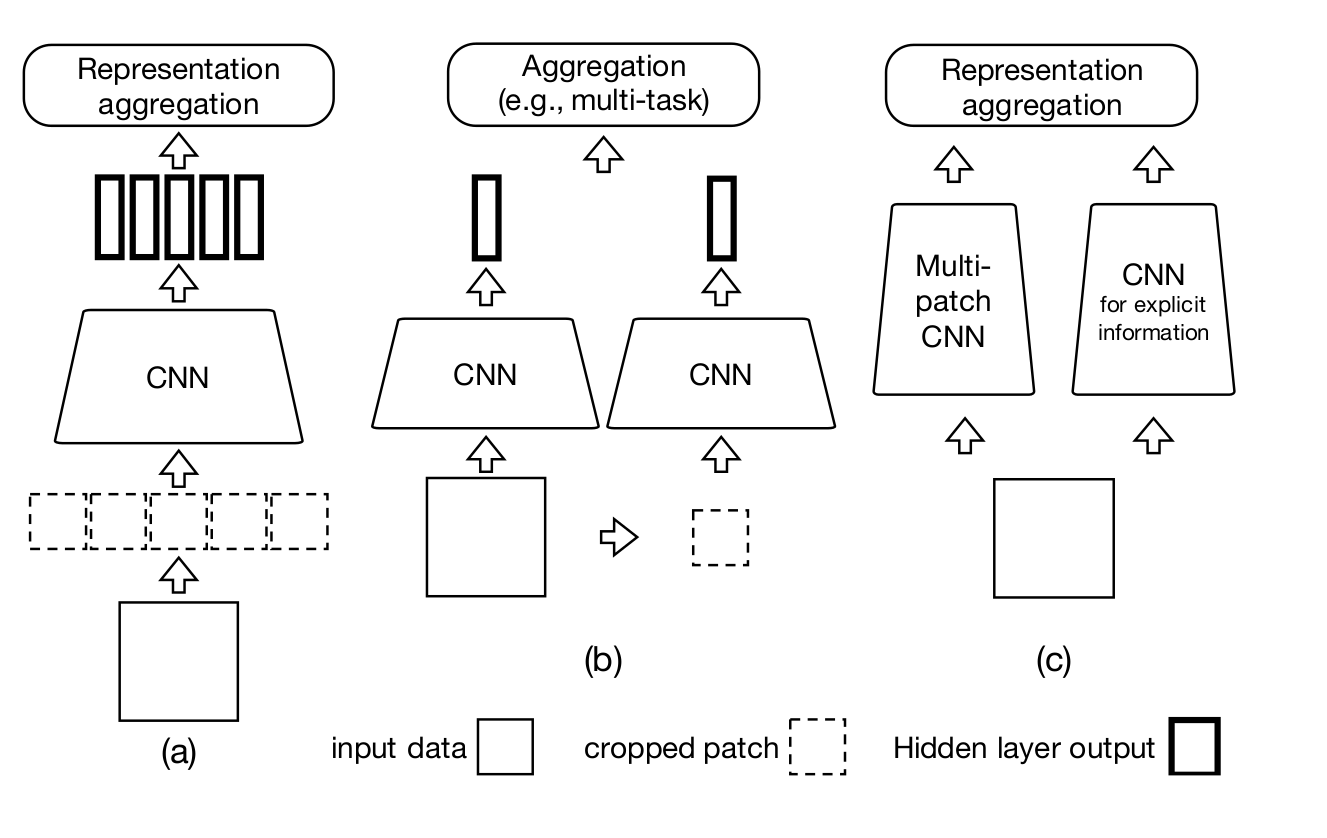
\includegraphics[width=0.3\textwidth]{figures/Literature Review/newtworks/Sheng2018_attention_based_MP.png}
    \caption{Aggregation based architectures for IAQA  \cite{Sheng2018}}
    \label{fig:MPADA}
\end{figure}


\subsubsection{Attention mechanisms} 
\label{sec:attention machanisms}

All of the state of the art models considered here are produced using attention mechanism or multi layer architectures that have been used to successfully improve classification accuracy, and produce models that perform better than vanilla networks on the AVA test set. 

Some of these approaches, such as A-Lamp \cite{Ma2017}, use adaptive patch selection based on the most informative patches, using graph based salience detection, to select multiple patches shown in figure \ref{fig:graph_patch}. 

Various iterations of this have been the rule within recent IAQA literature, and these have been to solve a range of technical challenges, which fall into the categories of \textit{spatial com positional, spatial intentional and semantic}. 

Spatially based attention is developed as a learning policy by \cite{Sheng2018}, who employs an optimisation strategy to maximise training accuracy by selecting new patches and avoiding bounding box coordinates of the previous patch for n attempts. Other attempts have sought to create a policy where a model can focus on aesthetically similar images \cite{Schwarz2018a}. 

Some have cropped salient patches a without any other transforms and built an attribute relation graph \cite{Ma2017}. The most recent and sophisticated of these create and utilise aesthetic related attributes and spatially related regions\cite{She_2021_CVPR} or use multi-modal approaches\cite{Zhang2021d} that leverage comments and information to combine self attention with attention based on LSTM trained on said comments. 

The latter two approaches mark the the most significant improvements in overall accuracy in the AVA bench marking, and represent a leap of significant margin. One drawback of these approaches is that they do not necessarily lend themselves to easy application, and are difficult to validate. Further, each approach somewhat reinvents the wheel in terms of attention mechanisms; none of these approaches have used a vision transformer or hybrid \textit{Convolutional Vision Transformer (CvT)} network.  

\subsubsection{Image Patching}
\label{sec:image patching}
%%%%%%%%%%%%%%%%%%%%%%%%%
% include eg from alamp %
%%%%%%%%%%%%%%%%%%%%%%%%%
The mean image size of the AVA dataset is $629 \times 497$ pixels with a maximum of $800^2$ pixels. The convention in almost all of the approaches sub-sample, down-sample, or crop images as part of data augmentation. This is often the first process in image augmentation; image patches are in most cases $3\times224\times224$, however, in some cases images have been warped to square before patching \cite{She_2021_CVPR} and others have been zero-padded to preserve composition. 


\begin{figure}
    \centering
    \begin{subfigure}[b]{0.25\textwidth}
        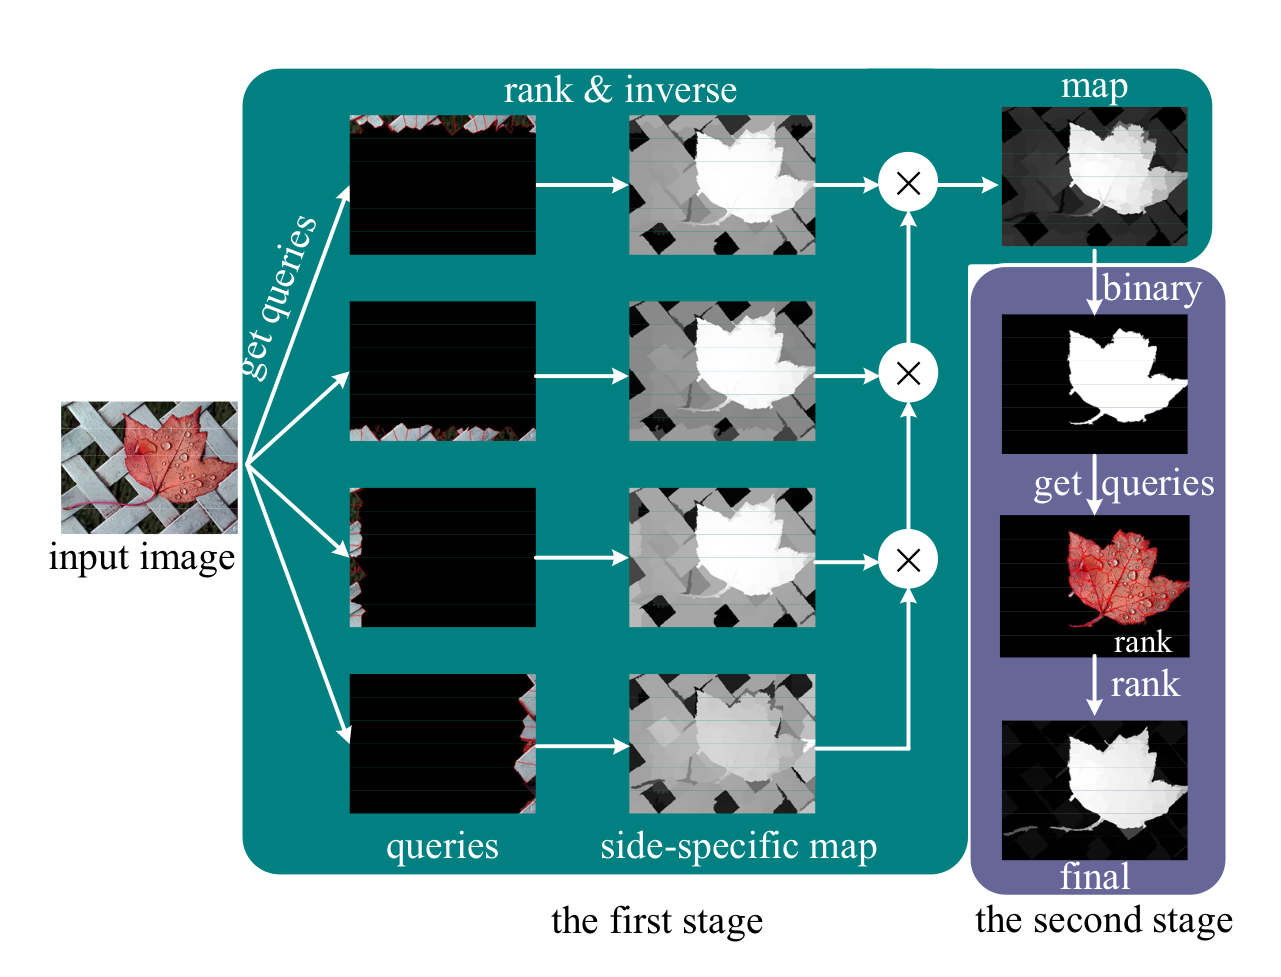
\includegraphics[width=\textwidth]{figures/Literature Review/yang2017_graph_based.png}
        \caption{Patching Example From Hand-Crafted Features \cite{Yang2013}}
        \label{fig:graph_patch}
    \end{subfigure}
    \hspace{5mm}
    \begin{subfigure}[b]{0.3\textwidth}
        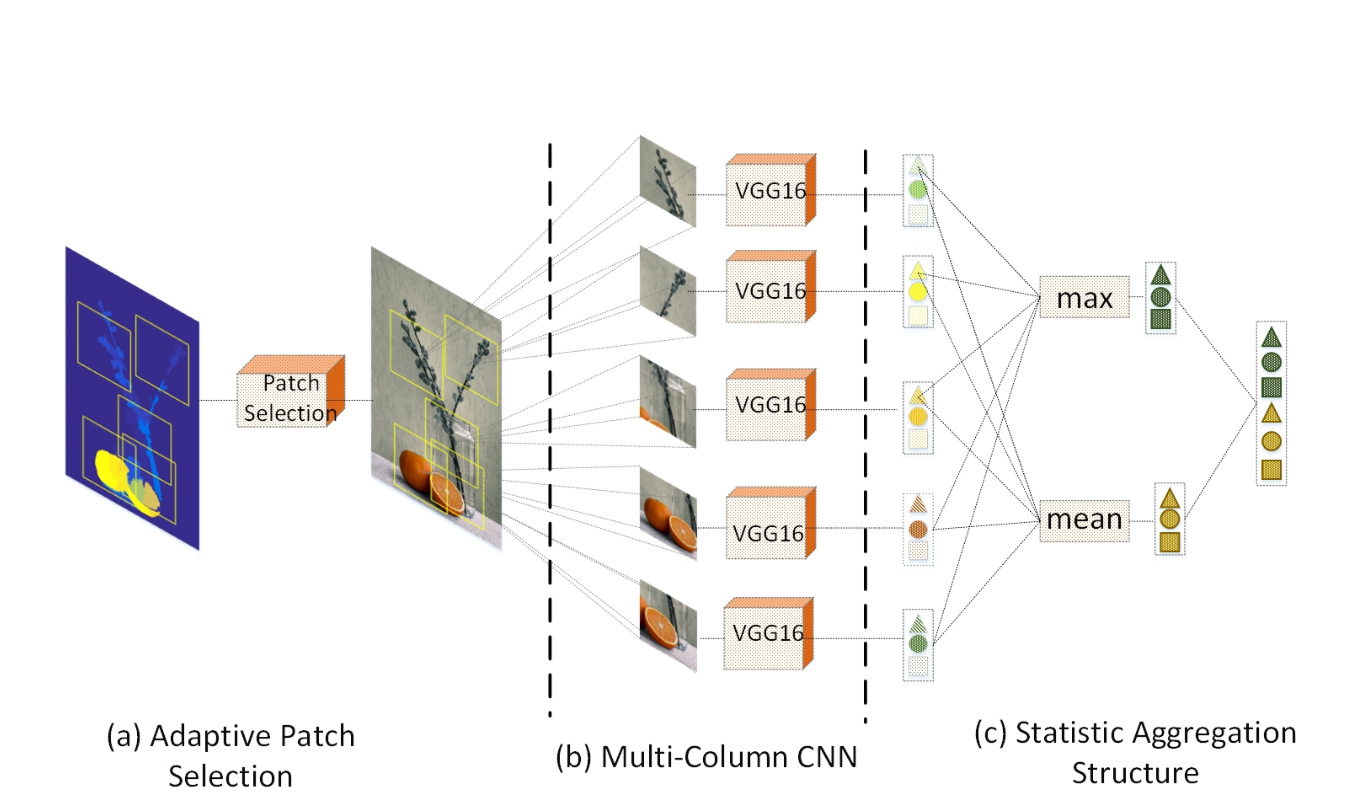
\includegraphics[width=\textwidth]{figures/Literature Review/alamp_patch.png}
        \caption{A-Lamp Multi Patch Network  \cite{Ma2017}}
        \label{fig:alamp_multi}
    \end{subfigure}
    \hspace{5mm}
    \begin{subfigure}[b]{0.25\textwidth}
        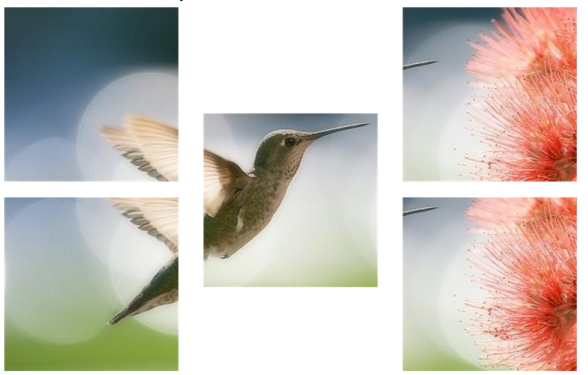
\includegraphics[width=\textwidth]{figures/Literature Review/alamp_bird.png}
        \caption{Patches Taken From AVA Dataset Based on Saliency Graph \cite{Ma2017}}
        \label{fig:alamp_patches}
    \end{subfigure}
    \caption{ Patching Examples from Hand-Crafted \cite{Yan2013} and Deep Features   \cite{Ma2017}}
\end{figure}



\begin{table}[ht]
\tiny
    \centering
    \begin{tabular}{c?p{2cm}ccp{2.5cm}c }
 \specialrule{.1em}{.1em}{.1em}
 \multicolumn{6}{c}{*State of Art Models and Metrics on AVA Dataset*}\\
 \specialrule{.1em}{.1em}{.1em} 
  \textbf{Year} $\downarrow$  &  \textbf{Model} & \textbf{Reported Acc.} $\downarrow$ & \textbf{Reproduced Acc.} & \textbf{Approach} & \textbf{Backbone} \\
 \specialrule{.1em}{.2em}{.01em}
  2014 & RAPID DCNN\cite{Lu2014a}& 75.4        & -- & Double column CNN (texture) & AlexNet\\
  \specialrule{0.01em}{0.1em}{0.1em}
  2015 & DMA-Net \cite{Lu2015b} & 75.4 & -- & Multi-column & Alexnet\\
  \specialrule{0.01em}{0.2em}{0.1em}
  2016 & A\&C CNN\cite{Kao2016} & 74.5      & --& Scene Object Texture (multi attr./col.) & Rapid CNN\cite{Lu2014a} \\
  \specialrule{0.01em}{0.2em}{0.1em}

  2016  &  MNA-DCN\cite{Mai2016}    & 77.1     & -- & Adaptive Spatial Pooling  &  VGG-16\\
  \specialrule{0.01em}{0.1em}{0.1em}
  2016 & MNA-CNN-Scene\cite{Mai2016} & 77.4 & --& Multi-Column (spatial)  & VGG16 \\
 \specialrule{0.01em}{0.2em}{0.1em}
  2016 & BDN\cite{Wang2016c}     & 78.9     & --& Multi column (directed augmentation)   & Custom Auto Encoder    \\
  \specialrule{0.01em}{0.2em}{0.1em}
  2016 & MTCNN \cite{Koa2016b} & 79.1 & -- & Baysian Multi Task  & AlexNet, VVG Net, ResNet\\
  \specialrule{0.01em}{0.2em}{0.1em}
  2017  &  New-MP-Net\cite{Ma2017}    & 81.8     & -- & Multi-Patch     & VGG-16\\ 
  \specialrule{0.01em}{0.2em}{0.1em}
  2017 & MultiGap\cite{Hii2017a} & 82.27 & -- & Multi pooled with text augmentation & GoogLeNet\\
  \specialrule{0.01em}{0.2em}{0.1em}
  2017 & A-Lamp\cite{Ma2017} & 82.5        &-- &  Adaptive-Multi patch (spatial)  & VGG16\\
  \specialrule{0.01em}{0.2em}{0.1em}
   2018 &   NIMA \cite{Talebi2018} & 81.51    & 77.36  & Reproduces MOS Distribution & Inception-v2, MobileNet\\
  \specialrule{0.01em}{0.2em}{0.1em}
    2018 &   MPADA\cite{Sheng2018}        & 83.03    & 79.1   & Attention Based Multy-Patch & Resnet18\\
  \specialrule{0.01em}{0.1em}{0.1em}
  2019  &  MLSP\cite{Hosu2019}          & 81.72    & 81.7   & Double column CNN &VGG-16 \\
  \specialrule{0.01em}{0.2em}{0.1em}
    2020 & AFDC\cite{Chen2020b} & 83.2 & -- & Muli-column adaptive mini-patch & ResNet50, VGG16\\
  \specialrule{0.01em}{0.2em}{0.1em}
  2020 & FCN-A-G\cite{Liu2020} & 83.6  & -- & Region Graph Convolution (fully conv.)  & Resnet101 FCN, VGG-16, DenseNet-121\\
  \specialrule{.1em}{.1em}{.5em}
  2020 & PA IAA\cite{Li2020a} & 83.7 & -- & Siamese Multi-column & Densnet121, Inception-V3\\
  \specialrule{0.01em}{0.2em}{0.1em}
  2020 &   MSCAN \cite{Zhang2021d}       & 86.66    & -- & Multi Modal Self colab. attnt. & VGG16   \\
  \specialrule{0.01em}{0.2em}{0.1em}
   2021 & HLA-GCN\cite{She_2021_CVPR} & 84.6 &  -- & Layout-Aware Graph CNN & Resnet-50, Resnet-101\\
  \specialrule{0.01em}{0.2em}{0.1em}
\end{tabular}

    \caption{State of The Art Metrics (overall accuracy)}
    \label{tab:SOA}
\end{table}

\subsection{Hand-Crafted Features Genealogy}
\label{sec:handcrafted} 

The approaches within IAQA fall into two main categories: hand-crafted (HC) and so-called deep features. HC features are extracted at both \textit{lo} and \textit{high} level and are extracted by traditional approaches to digital image processing\cite{gonzalez2008digital}. 

%%%%%%%%%%%%%%%%%%%%%%%%%%%%%%%%%%%%%%%
% SHOULD THIS INCLUDE A LEVEL EXAMPLE %
%%%%%%%%%%%%%%%%%%%%%%%%%%%%%%%%%%%%%%%





\subsection{Feature Extraction}
\begin{table}[ht]
\tiny
    \centering
    \begin{tabular}{c?p{2cm}p{2cm}p{2cm}cccc}
        \specialrule{.1em}{.1em}{.2em} 
        \multicolumn{7}{c}{* Chronology of IAQA Techniques*}\\
        \specialrule{.1em}{.1em}{.2em} 
        Date & Technique & Feature Type & Extracted (imaging process) &  Feature Levels $\ddag$ & Dataset & Metric & Score\\
        \specialrule{.1em}{.1em}{.2em} 
        2004 & Ada-Boost, Real-AdaBoost (SVM, Bayesian) Classifier\cite{Tong2004} & Texture, Shape, Color, Energy & Band Diff. color histogram, color moment, lab coherence, HSV Coherence, DFT Moment,DCT moment, Wavelet, hist $\in \{Sobele, Laplace, Canny\}$, &  H/L & B$\dagger$ & Linear Corr. & 84.7\% \\ 
        
        \specialrule{0.01em}{0.2em}{0.2em}
        2006 & SVM Binary Classification\cite{Datta2006}& Texture, Familiarity, Size, Depth of field & Wavelet Based and 56 subset functions & H/L & P.Net & ACC  & 70.12\% \\ 
        \specialrule{0.01em}{0.2em}{0.2em}
         2006 &Naive Bayes class \cite{Ke2006}& Glob Edge Distribution, Color Dist., Lo-level Contrast, Brightness indicator   & Laplace Filter, KNN, 20bin Histogram, Fourier Transform & H/L& DPC & ACC & 72\% \\
        \specialrule{0.01em}{0.2em}{0.2em}
        2008 & SVM, Gentle ADABoost, Bayes Classifiers\cite{Lou2008} & clarity, contrast, lighting, simplicity, composition geometry, color harmony & Histogram, blurring kernel, $f(Hue \times Bri. \times Sat.)$& H/L & DPC & max AUC &  $93\%$\\
        \specialrule{0.01em}{0.2em}{0.2em} 
         2009  & SVM Classifier\cite{Wong2009}& salient object, subject background  & Saliency Map  & H/L & P.Net &  5CV-ACC & 78.8\\
        \specialrule{0.01em}{0.2em}{0.2em}
        2011&SVM Classifier \cite{Dhar2011}&Colour, DOF, Illumination of sky & Color spatial dist., multi scale contrast, Wavelet Energy, Haar Features, Spatial Pyramid Shape &H/L &DPC/Flkr. & ROC & -- \\
        \specialrule{0.01em}{0.2em}{0.2em}
        2012 & SVM Classifier\cite{Lo2012a} & Layout, Composition, Texture, color& Hist, FFT, kNN(color) & H/L & CUHK &  mean ACC &  86\%\\
        \specialrule{0.01em}{0.2em}{0.2em}
        2013 & SVM Classifier\cite{Tang2013a} (feature prediction) & Geometric composition, Complexity, DOF, Hue Composition, Blur, Brightness & Color harmony $f$, Orientation $f$, Salience map, Kernel Blurring &  H/L & CUHKPQ & max AUC &  $<80\%$\\  
        \specialrule{0.01em}{0.2em}{0.2em}
         2015 & Bayesian Network Support Vector Regression (SVR)\cite{Gao2015a}&17 High level & SSIM, SIFT, HOG &  G & DPC/PNet &ACC & 72.7 &\\
        \specialrule{0.01em}{0.2em}{0.2em}
         2015&SVM  Classifier \cite{Mavridaki2015}&  Proposed
         Simplicity, Colorfulness, Sharpness, Pattern, Composition & Histogram Wavelet coefficients, Euclid distance, Color histogram & H/L& CUHK-PQ/AVA & ACC & 77.1\% \\
        \specialrule{0.01em}{0.2em}{0.2em}
        2016 &SVM \cite{Wu2016}  &  Aesthetic Class & mulitmodal,Structural Features, Local Vision features, Functional purpose& H & DS2 &ACC & 78.42\\
        \specialrule{.1em}{.1em}{.2em}
        \multicolumn{7}{c}{$\ddag$ High(H) Low(L) Features, $\dagger$ Bespoke} \\
        
\end{tabular}
    \caption{Approaches to Feature Extraction}
    \label{tab:IAQA Approaches}
\end{table}

Early approaches to IAQA combined 'low-level' features and processes, such as wavelet transforms, to obtain image texture to 'extract' information, or applied coefficients recursively to obtain edge information, or applied some coefficient across an image to compute blurriness. 

The trend in the use of HC features seems to be from multiple complex and individually defined functions, for example \cite{Datta2006} and \cite{Tong2004}, (early examples) both of whom extract 56 and 15 individual features respectively and later examples \cite{Gao2015a} extract only three but apply a more complex learning algorithm. 

\subsubsection{Global/Local}



Almost all approaches use both global features such as texture, and local features such as salient objects. There is some ambiguity in the literature about what constitutes 'local'. Examples of a low-level features are sub-banding in Wavelet, convolving across images, where there is therefor some spatial locality or granularity to the extracted feature. 

\subsubsection{Pipeline}

Many of the features are highly complex functions that have relied on the knowledge of signal processing and making use of Fourier spectrum transforms\cite{Ke2006}, as well as other are more simple histogram calculations (where pixel values are binned into hues) to calculate color harmony.

Figure\ref{fig:handcrafted} shows a typical HC feature extract-on and SVM training pipeline. 

Many of the HC feature extraction approaches reviewed here grouped various features into categories or types such as composition\cite{Lou2008} or blurriness\cite{Ke2006}. Extraction in the design is that of crafting, using engineering skill and domain knowledge to select the design features that correlate with image quality.  

    \begin{figure}[ht!]
    \centering
    \specialrule{0.01em}{0.2em}{0.2em}
    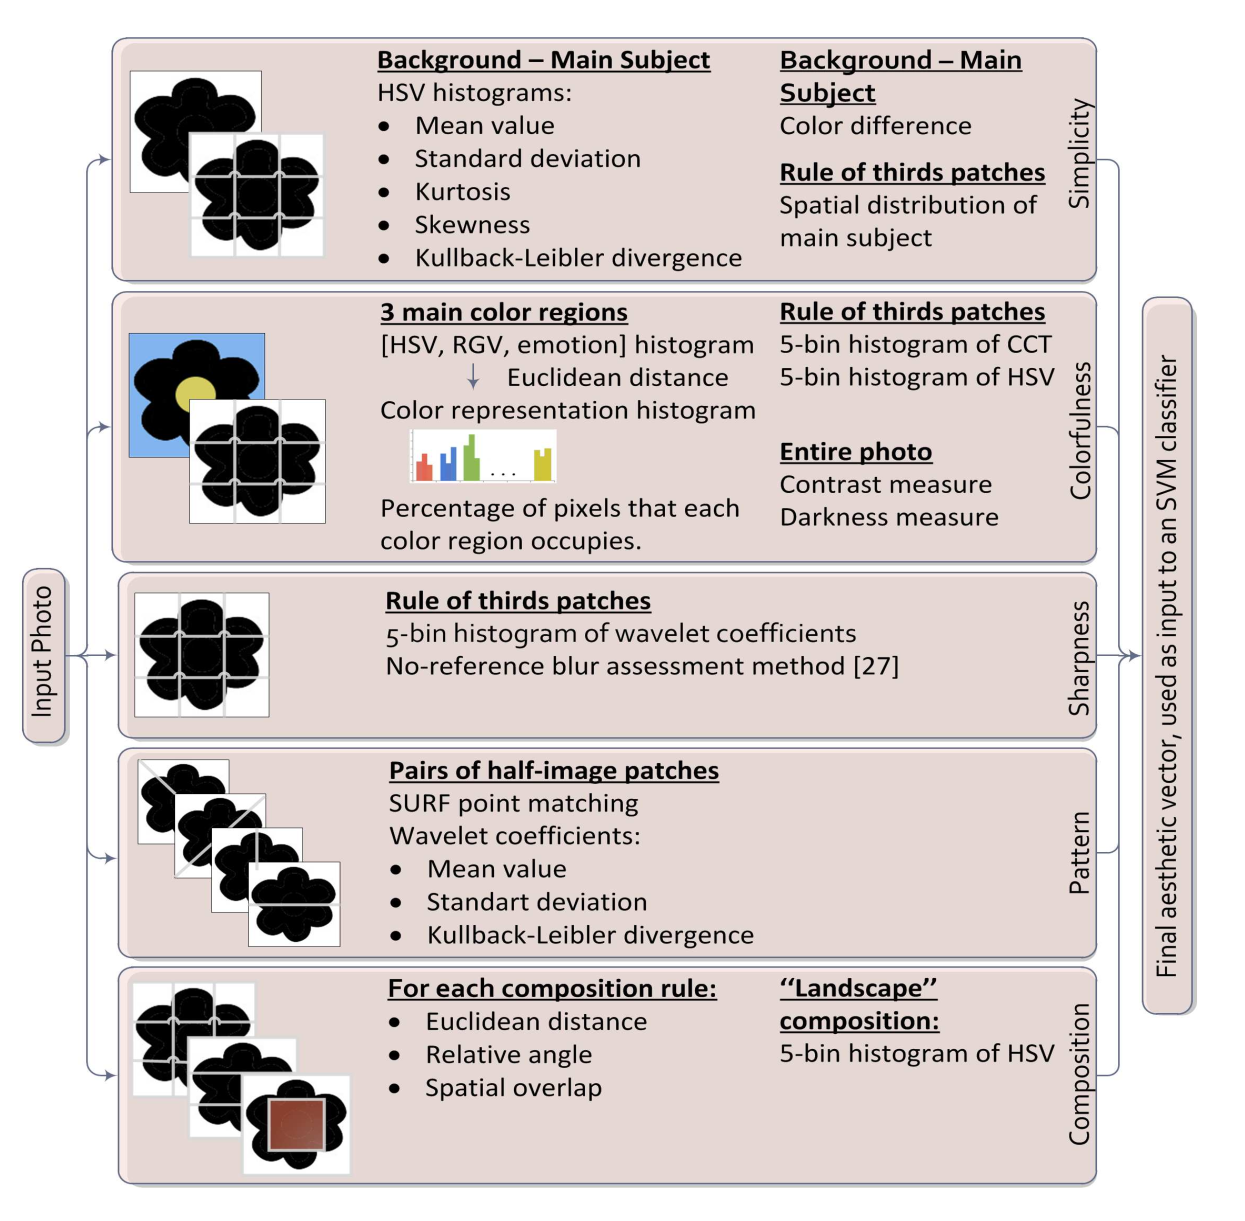
\includegraphics[width=0.5\textwidth]{figures/Literature Review/Hand_crafted/Mavridaki2015_pipline.png}
    \caption{Hand-crafted feature extraction pipeline \cite{Mavridaki2015}}
    \label{fig:handcrafted}
    \specialrule{0.01em}{0.2em}{0.2em}
    \end{figure}

\subsubsection{Convolutionally \emph{or} Conventionally Derived Features}

Approaches, such as convolution operations, which were formerly a mode of implementing a process of applying a predefined coefficient, have shifted to become fundamental and dominant attributes of deep learning for computer vision. 

Deep learning inverts this, making the convolution operator central and neglecting such aspects as high or low-level features, domain expertise, or fundamental understanding of physical properties, which image processing requires. Within this, it is interesting to note that more recent HC feature driven approaches tend to favour simple features and complex image categories\cite{Mavridaki2015,Gao2015a}, perhaps in response to deep learning's dominance? 

Further, of the HC approaches comprehensively reviewed and shown in Table \ref{tab:IAQA Approaches} only one compared results with the AVA dataset \cite{Mavridaki2015} where side-by-side accuracy is 0.77\% on a subset of only top and bottom 10\%(score 1 and score 10) quality images(ignoring 80\%) of data including most ambiguous images. The most accurate binary classification HC approaches were trained on Chinese Hong Kong University-Picture Quality (CUHK-PQ) dataset\cite{Lo2012a}. This dataset is heavily annotated, and has had expert input in rating high and low quality, in addition to being much smaller. All approaches have performed well on this dataset of professional images. 

\subsection{A Case for Deep Learning}
\label{sec:a case for dl}

There is clearly a great deal of interlinking between categories, such as object emphasis, the 'rule of thirds', and shallow DOF, such that a point of focus or object emphasis might be achieved through rule of thirds or shallow depth of field which are categories defined, for example, in the AADB (Aesthetics Attributes Data Base) ( section \ref{iaqa datsets appendix} figure \ref{fig:AADB_1})  with GT labels and HC features. Even 8 HC features can result in a great deal of complexity and ambiguity - not withstanding the high degree of human interpret ability of such concept as a 'balanced element'.

\begin{figure}[ht!]
\specialrule{0.01em}{0.2em}{0.2em}
\centering

\subfloat[${I}\cup{B} \subseteq{O} $]{
  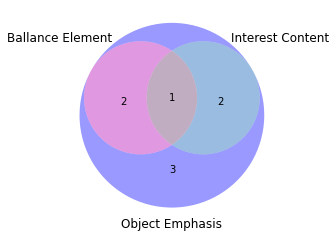
\includegraphics[width=0.2\textwidth]{figures/AADB/feature_venn.png}
  
}
\subfloat[${I}\notin {B} \notin{O} $]{
  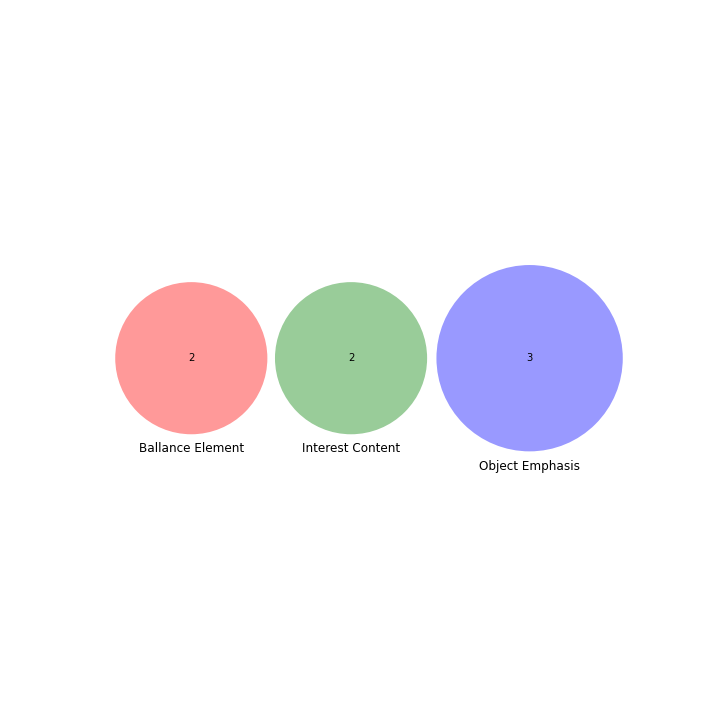
\includegraphics[width=0.2\textwidth]{figures/AADB/disjoint.png}
}
\hspace{1mm}
\subfloat[${I}\cup{B} \cup{O} $]{
  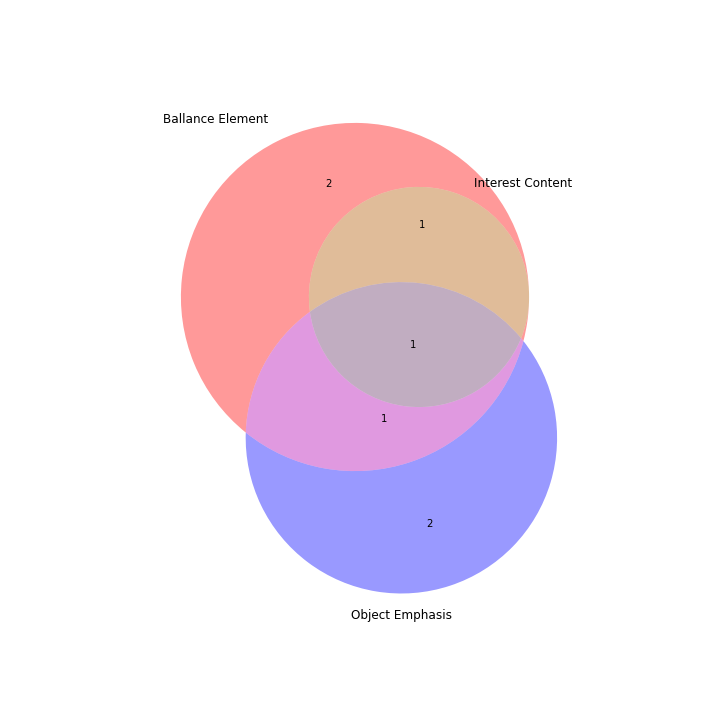
\includegraphics[width=0.2\textwidth]{figures/AADB/high_intersection.png}
}
\subfloat[${I}\subseteq{B} \subseteq{}{O} $]{
  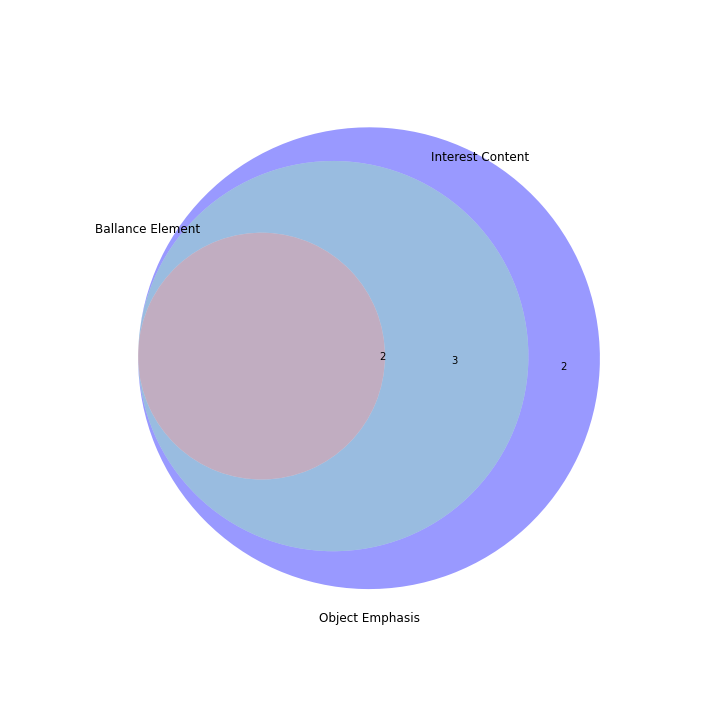
\includegraphics[width=0.2\textwidth]{figures/AADB/recursive_intersection.png}
 
}

\caption{\label{fig:AADB_Venn}4 Possible configurations of inter-dependant features within sample space of 8 possible features}
\label{fig:AADB_Venn_}
\specialrule{0.01em}{0.2em}{0.2em}
\end{figure}

This process as has a high-branching factory and  ${\binom{n}{k} = \frac{n!}{k!(n-k)!}}$  possible subsets ${\binom{n}{k}}$ where n is the number of features n and k is number definable or possible features \textit{feature space} that constitute a high quality image. In a search space of $x \in \mathbb{Z} \times 2^{8^{(n \times m)}}$ this is clearly a high number. 

This has the drawback of reliance on human pattern recognition and human defined features, to which machine learning is then applied. In removing the need to define features by hand \textit{a priori}, deep learning represents a paradigm shift and has several advantages for the IAQA domain: 


\par
   
\begin{itemize}

    \item Removal of human bias from feature definition, where definitions within aesthetics remain inherently ambiguous;
    \item Potential ability to generalise better;
    \item Finding patterns in image data that humans would not;
    \item Models can be used to predict image quality of new images easily. 
\end{itemize}

However, while the techniques employed on smaller datasets, such as AADB, may generalise less well on unseen data, HC approaches are appropriate for generating learning from a smaller databases. And approaches that combine both, such as \cite{Kong2016}, provide valuable insights for later analysis. These earlier forays into IAQA should not be disregarded. 
\newpage



\section{Related Data sets}
\label{sec:related_data} 

This section will provide an overview of the different datasets that have been used for IAQA. The purpose of this is to provide further detail, outline some of the inherent challenges, such as class balance within, and how to formulate a problem in such a way as to be able to effectively train and measure against benchmarks, and to illustrate the history and development of the field and draw out how new learning has been generated in previous work.\par

\begin{wrapfigure}[16]{l}{0.5\textwidth}
\specialrule{0.01em}{0.2em}{0.2em}
     \begin{center}
     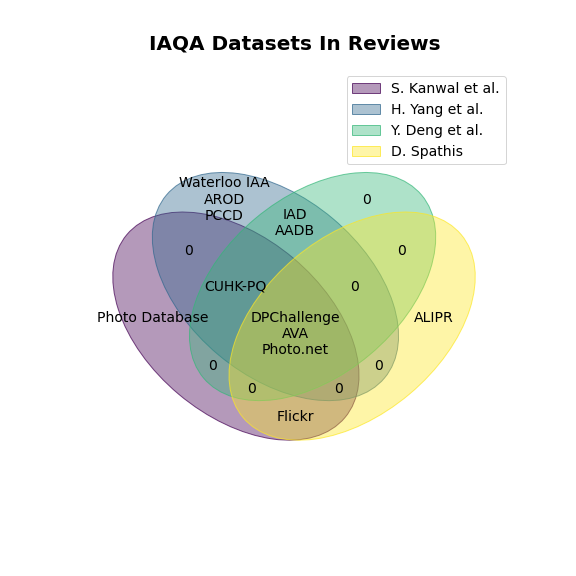
\includegraphics[width=0.45\textwidth]{figures/data_plots/datasets.png}    
     \caption{\label{fig:Data_venn} Venn diagram Datasets Reviewed in Literature Reviews}
     \label{fig:venn}
  \specialrule{0.01em}{0.2em}{0.2em}
  \end{center}
\end{wrapfigure}
Within the literature that surveys the IAQA domain, there are 15 datatsets (shown in Table \ref{Tab:IAQA Datasets}) that are reviewed in some capacity, and have had publications associated with them. There are also a number of publications that have formed their own bespoke datasets, or which are subsets of existing dataset. In IAQA Reviews \cite{Yang2019,Kanwal2021,Spathis2016,Deng2017}, there are 12 datasets covered. IAQA reviews consistently cover AVA and DPChallenge, however a significant number of datasets are only mentioned by a single source see \ref{fig:venn}, this is reflective of wider IAQA research. \par

Although their are many IAQA datasets,it is clear from the variability both in overall size and type of annotation that, while benchmarking datasets in other areas of computer vision, such as image classification (Cifar $\in\{10, 1000\}$\cite{Krizhevsky2009,Krizhevsky2009a}, ImageNet\cite{Deng2009} $\in \{1K,21K\}$ ), IAQA datasets  are less well defined and readily available. Within this, several subset dataset have been formed to address challenges such a minority class or sparsity of a super set have been compiled. 

\begin{table}[ht!]
\tiny 
    \centering
    \begin{tabular}{c|ccccc}
 \specialrule{.1em}{.2em}{.2em}
 \multicolumn{6}{c}{*Image Aesthetic Quality Assessment Data Sets*} \\
 \specialrule{.1em}{.2em}{.2em} 
 Name &Size \newline (n images) & Classes & Year & Additional & source \\
 \specialrule{.1em}{.2em}{.2em} 
AADB\cite{Kong2016}           & 10,000    & 2           & 2017  & 12 subsets  & Flk.      \\ %have paper
AROD\cite{Schwarz2018a}       & 304,000   & 2  & 2018  &             & Flk.          \\ %have paper \\ 
ALIPR\cite{Datta2008}         & 13,010    & 10          & 2018  & sentiment   & Flk.        \\ %have paper
AVA\cite{Murray2012}          & 255,530   & 10,2        & 2012  & discretized & DPC      \\ %have paper
CUHK-PQ\cite{Tang2013a}       & 17,690    & 2           & 2013  & 7 sub-cats  & DPC          \\ %have paper
DPChallenge\cite{Datta2008}   & 16,509    & 10          & 2008  &             & DPC         \\ %have paper
FCDB\cite{Chen2017}           & 4135      & $\infty$  & 2017  & cropping    & Flk.       \\
Flikr\cite{Yin2012,Chang2017} & 80000     & 2           & 2017  & geo-tagged  & Flk       \\
Flickr AES \cite{Ren2017}     & 40000     & 2           & 2012  &             & Flk.        \\ %have paperh 
IAD\cite{Lu2015a}             & 1,500,000 & 2           & 2014  &             & Multi       \\ %have paper
IDEA\cite{Jin2020}            & 9191      & 10          & 2020  & ballanced   & DPC          \\
PCCD\cite{Chang2017}          & 4135      & 7           & 2017  &             & Bespoke     \\
PD*\cite{Lo2013}  & 1051      & 2           & 2013  &             & CUHK-PK      \\ %have paper
Photo.net\cite{Datta2006}     & 3581      & 7,2         & 2010  &               & P.net   \\ %have paper
Waterloo IAA\cite{Liu2017a}   & 1000      & 7           & 2017  & discretized & P.net          \\ %have paper
 \specialrule{.1em}{.2em}{.2em}
 
\end{tabular}
\caption{IAQA DATASETS}
\label{Tab:IAQA Datasets}
\end{table}

Figure~\ref{fig:Data_venn} shows only three datasets of literature reviewers that are explicitly covered by in all four IAQA review publications( AVA, DPChallenge, and Photo.Net). The AVA Datasets is a super set containing DPChallenge images and is clearly central to the IAQA domain.

IAQA ground truth scores are described through the literature as a distribution MOS (Mean Observed Score). Some datasets have fewer ground truth voters - 28 votes per image photo.net \cite{Murray2012, Wu2011} and others have many raters from a single online community and have 210 per image (AVA); some are rated using a paid for service such as Amazon Mechanical Turk(AMT), or by specialist highly controlled informants where screen and demographic information are recorded in addition to image rating. 
 
 Dataset sizes range from 1100\cite{Liu2017a} Waterloo IAA to 1.4 million\cite{Lu2015a} images (IAD). The mean dataset size overview is 152k images. Figure \ref{fig:IAQA_Data} shows a plot of the dataset against the year of associated publication, and while there does appear to be small positive correlation, there is also an increasing degree of variability in dataset size, with both the smallest and largest datasets being first associated with publications only two years apart.
 \begin{figure}[ht!]
 \hrulefill
 \begin{center}
 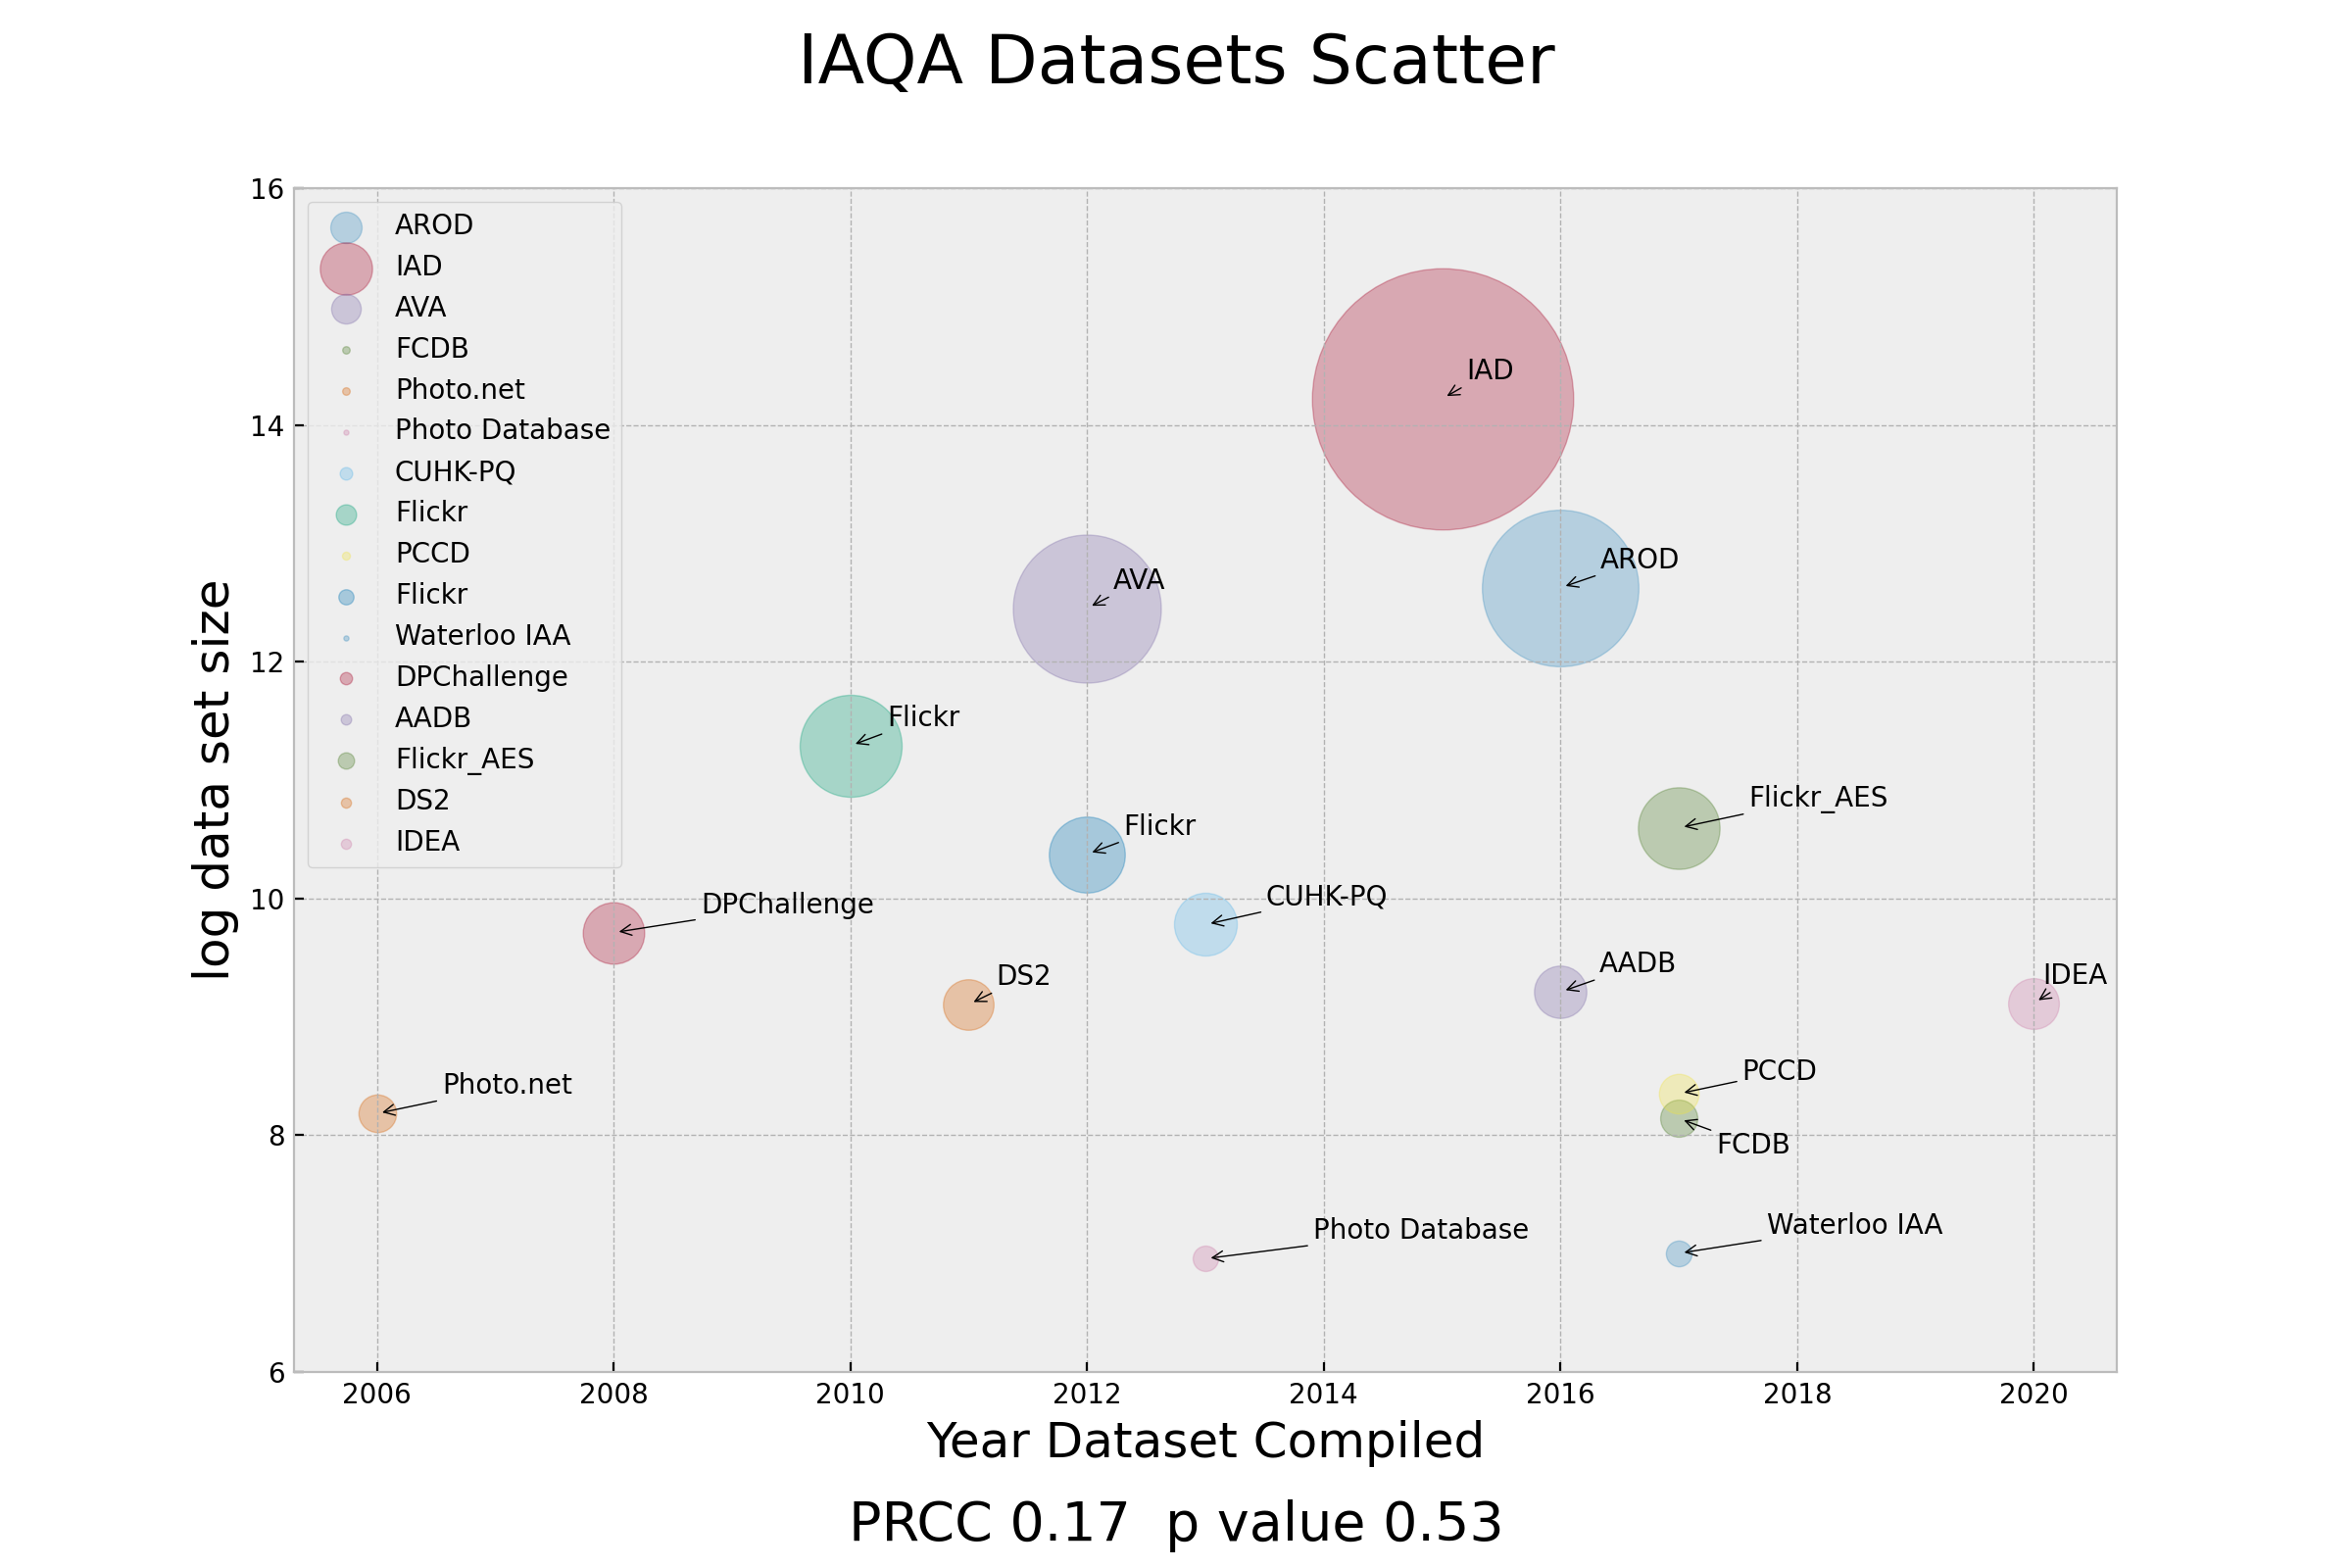
\includegraphics[height=0.55\textwidth]{figures/data_plots/iaqa_ds_size.png}
  \caption{\label{fig:IAQA_Data} Dataset Size and Year of Publication Plot}
  \label{fig:IAQA_Data_}
\hrulefill
 \end{center}
\end{figure}
 Further, this divergence seems to increase with time. While available data in other areas of computer vision appears to have increased with time, this is not the case for IAQA, where even very recent publications propose novel datasets such WaterlooIAA\cite{Liu2017}. There is no evidence to reject a null hypothesis that datasets do \textit{not} increase over time.
 
 The MOS distribution of IAQA datasets frequently appears Gaussian\cite{Murray2012, Datta2008, Yang2019, Talebi2018}. AVA is the most normally distributed of these\cite{Murray2012}, where a Gaussian probability density function is given by:

\begin{equation}\label{Gaussian PDF}
f(x) = \frac{1}{\sigma\sqrt{2\pi}} 
  \exp\left( -\frac{1}{2}\left(\frac{x-\mu}{\sigma}\right)^{\!2}\,\right)
\end{equation}



Where $\sigma$ is standard deviation and $\mu$ is mean MOS. The AVA dataset has the most normally distributed dataset of any available IAQA dataset to date\cite{Murray2012}, and has more than 300\cite{AVA2012} associated publications. This is significant in particular for the AVA dataset, where the mean number of votes for each image $ = 210$. This can be taken as a reliable ground truth value, where the probability of an image being scored on some scale is greatest at its mean and enables the exclusion of relatively few images as outliers from a normal distribution. 

Further, it is significant that within this AVA Database of $\approx 255k$ images, only a very small number are excluded as outliers, where an outlier is $\pm4\sigma$, which, while not in itself a test for a normal distribution, shows the normal test for an outlier is $\pm2\sigma$. \par 

This is  consistent with the notion of so called \textit{vox populi} or 'wisdom of crowds' and was initially researched and coined by F. \citeauthor{Galton1907}\cite{Galton1907} in his significant demonstration that mean estimated values of crowds were frequently within $\pm3.1\%$ of ground truth (GT)\footnote{Frances Galton would likely not have used the term ground truth}. 

This significant finding provides a sound reasoning for aggregating crowd sourced scores as a measure of actual image accuracy. One aspect that is not taken into consideration with approximating GT, however, is online community bias, and one point of critique of the AVA dataset is that individual users are not identified and it is further not possible identify how individual users vote over time across different images, or conversely how an online community might vote for different images of the same user.\par 

Classification tasks, which many IQAQ publications employ as routine throughout the literature, compute MOS of each image and then threshold this into usually good or bad image quality categories. This, however, results in class imbalance with the low category as a minority class. The practice of computing MOS (see eq. \ref{mos}) emerged in IQA where HC and traditional computer vision approaches such as\cite{Wang2004} were employed as proxies for GT. 

\begin{figure}[ht!]
\specialrule{0.01em}{0.2em}{0.2em}
\centering
 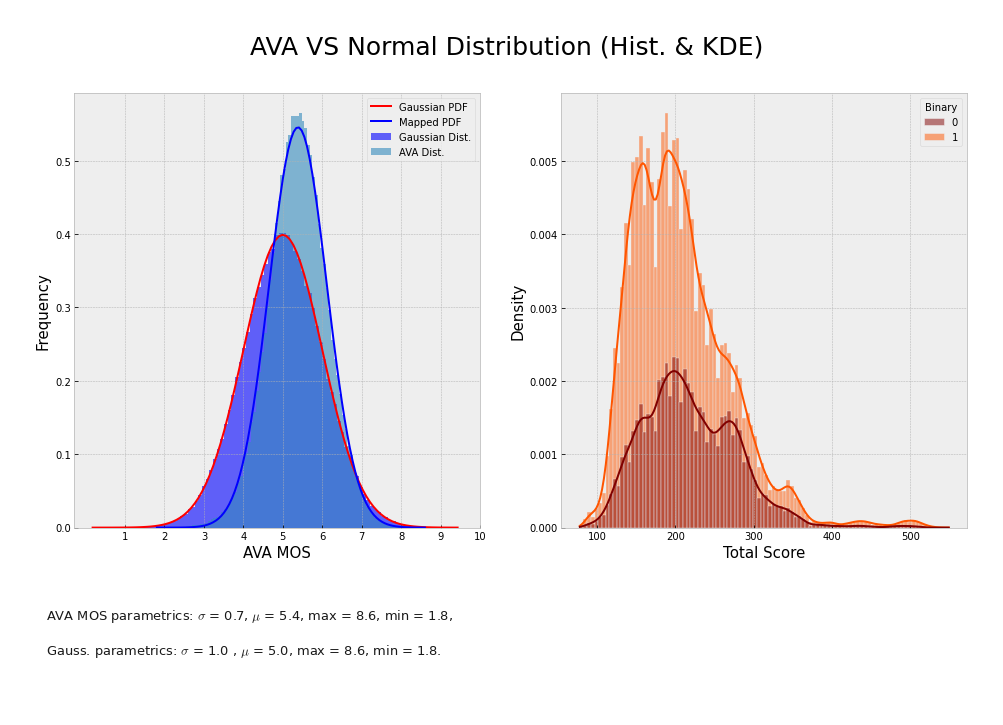
\includegraphics[width=0.65\textwidth]{figures/data_plots/ava_paramiters_gt.png}
  \caption[width=0.5\textwidth]{\textbf{Left} Compared Gaussian with AVA Distribution of MOS Scores with Gaussian PDF as Defined Above in  \textbf{Right} and Kernel Density of Score: low (0) and high (1)}
  \label{fig:AVA_MOS}
\end{figure}


 Figure \ref{fig:AVA_MOS}, left, overlays plots of gaussian distribution and the AVA dataset (light blue). The line's Probability Density Function (PDF) of a gaussian distribution e.q. \ref{Gaussian PDF} (red) and a computed PDF mapped to AVA MOS scores showing a slight positive skew. The main deviation from this is in values around the mean (note histogram bars above blue PDF). 
 \par 
 
 One potential source of error aggregating human ratings is that it is not possible to rate 0, but it is possible to rate an image at 10. This may account for some psychological bias when rating images . Figure \ref{fig:AVA_MOS} \textbf{right}  appears corroborate this, with the positive scores outnumbering the negative scores and also showing less normalcy of distribution. Figure \ref{fig:AVA_corr} shows that as the number of votes increases, the average score appears to increase with it. 
 
\begin{figure}[ht!]
\centering
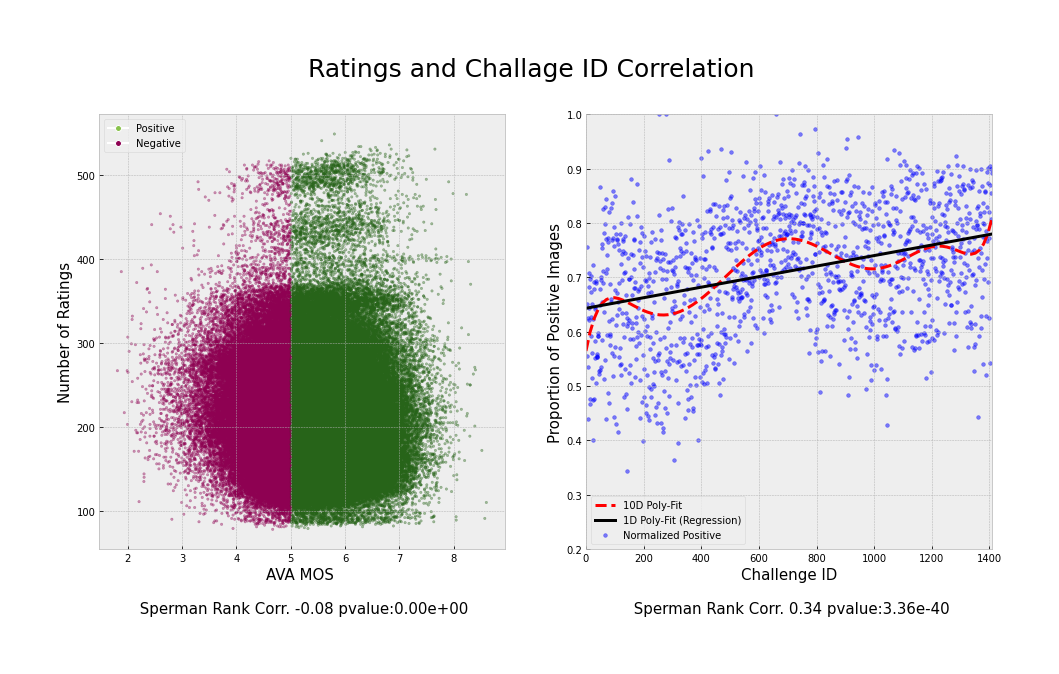
\includegraphics[width=0.65\textwidth]{figures/data_plots/MOS_rating_corr_gt.png}
 \caption{ Number of Ratings MOS Correlation \textbf{left} Proportion Positive Correlation with Challenge ID $\Delta T$ \textbf{Right} (With 10 Dimensional Polynomial Fit(Red)}
 \label{fig:AVA_corr}
 \specialrule{0.01em}{0.2em}{0.2em}
\end{figure}

Figure \ref{fig:AVA_corr} \textbf{left} shows both class imbalance (greater high than low) and an apparent increasing proportion of positive score with time. While time is not recorded, with Challenge ID (which increases monotonically) each challenge is opened and closed for a discrete time period. Therefore, it can be shown that there is a positive correlation with change in $\Delta T$ \ref{fig:AVA_corr} \textbf{right} with Spearman's Rank Correlation Coefficient (SRCC) of 0.34 and p value of $3.36 \times 10^{40}$ (this is almost certainly significant).\par 

Accounting for this could take a variety of hypotheses, such as a developing online community within dp.challenge.com. It is certainly clear from reading the comments on dp.challenge.com that there is an apparent social network with many members being persistent - this positive drift could be as a result of cognitive bias? \par 

While some datasets, such as AVA, consist of 250k images (which may have been considered large at its inception), when compared with domains such as object recognition where models can be trained on datasets such as Image-Net (which contains 15 million  images\cite{He2015a}) the available datasets for IAQA remain relatively small. Within the wider field of IAQA, which includes moving images, quality assessment, and fascinating areas such as calligraphy. 

Further, it is important to make a distinction between the field of image quality assessment (IQA) where benchmarking datasets such as LIVE IQA\cite{Ghadiyaram2016} represent images that have been degraded by artificial noise and are used as benchmarks for the sub-field of image restoration within computer vision. 


%%%%%%%%%%%%%%%%%%%%%%%%%%%%%%%%%%%%%%%%%%%%%%%%%%%%%%%%%%%%%%%%%%%%%%%%%%%%%%%%%%%%%%%%%%%%%%%%%%%%%%%%%%%%%%%

%subsection of baseling a

\section{Evaluation Metrics}
\label{sec:evaluation_metrics}

Almost all review approaches to IAQA are binary classification, with few treating as a ten class (reproducing probability distribution of images). 

For classification accuracy, balanced accuracy, and F1 score are reported within the literature; 'accuracy' is the most frequently used metric in IAQA literature\cite{Koa2016b,Schwarz2018a,Lu2014a,Ma2017,Chen2020b,Zhang2021d}. Much less frequent is balanced accuracy\cite{Deng2017} and F1 score by \cite{Ma2017, Mai2016a}. Many approaches use both regression and classification.  

\subsubsection{Accuracy}

'Accuracy' is a measure widely used to evaluate model performance in classification tasks, on both evaluation and test sets. 

\begin{equation}
    Accuracy = \frac{TP+TN}{TP+TN+FP+FN}
\end{equation}

\subsubsection{Balanced Accuracy}

This metric is particularly important in evaluation during the training and testing of models where there is a class imbalance, which is a significant attribute of many IAQA datasets. 

Balanced accuracy in the binary\footnote{for non binary cases, class weights must be computed} case used within IAQA is given by computing the arithmetic mean of sensitivity and specificity False Positive Rate (FPR)(eq.\ref{fpr}) (where sensitivity or true positive rate (TPR) (eq.\ref{tpr}):

\begin{equation}
    Balanced = \dfrac{FPR+TPR}{N_c}
\end{equation}
Where $N_c$ is the number of classes,TPR is given by:
\begin{equation}
    TPR = Sensitivity = \frac{TP}{TP+FN}
    \label{tpr}
\end{equation}
 and FPR is given by: 
\begin{equation}
    FPR = 1 - Specificity = \frac{FP}{TN+FP}
    \label{fpr}
\end{equation}
Other approaches to addressing class imbalance during training and evaluation are discussed below in the Methodology section.


\subsubsection{F1}

F1 score produces the harmonic mean of precision (eq. \ref{precision}) and recall (eq. \ref{recall}) and is given by: 
\begin{equation}
   F1 = \frac{2(Precision \Recall)}{Precision+Recall} = \frac{2(TP)}{2(TP+FP+FN)} 
\end{equation}

where precision is given by:

\begin{equation}
    Precision = \frac{TP}{TP+FP}
\label{precision}
\end{equation}


and recall is given by:

\begin{equation}
Recall = \frac{TP}{TP+FN}
\label{recall} 
\end{equation}

The evaluation metrics outlined here are for binary classification, but a number of approaches train a regression problem first, or compute the mean softmax of ten classes (reproduced score distribution) and use Persons Linear Correlation(PLCC) eq. \ref{PLCC} Coefficient or Spearman's Rank Correlation Coefficient (SRCC) \ref{SRCC}. 

This approach enables distribution analysis also, however it is not always clear in the literature whether a model has been trained purely as a regression model (reproducing MOS). Further, training a ten class problem is less challenging and does not give a good or bad quality estimation. This is particularly apparent with some of the more recent publications that achieve the highest accuracy training models with 10 node output of a fully connected layer. 

In order to be able to produce an end to end network here, we train a binary classifier rather than thresh-holding output computed MOS which approaches such as \cite{Talebi2018,Zhang2021d} appear to take. 


%%%Use your literature review to help the reader to understand the value and the interest in your project.  You should look for related works already published that either support the merit of your project, or provide the background understanding/information to make your new claims.  Try to avoid writing a "catalogue" of related works (e.g this would have little of your own insight added).  Instead, describe to the reader why the related work is interesting or relevant to your own work.  What did they achieve?  What did they overlook?  It is highly recommend you finish your Literature Review with a final subsection "Summary", where you may wish to formulate highly specified research questions or hypotheses, or assert the need for your Research Methodology (next chapter).  

\section{Literature Review Summary}



We show that deep learning has surpassed HC feature extraction on large dataset where IAQA is a binary classification problem and outline why we conduct experiment on the AVA dataset. The role of image processing is now part of data augmentation, however many of the HC approaches provide valuable insights into IAQA features, in part as they require a human understanding of the domain. Deep learning inverts this, making convolution operator central rather than a method of feature extraction, secondly the process of making predictions beyond good or bad is more more straightforward with HC approaches where individual aesthetic attributes can be defined, extracted with a greater degree of explainability. 

While many of the deep learning approaches outperform HC reliant feature extraction, deep learning approaches rely on hand crafting of complex learning policies on equally complex multi column network architectures.


We also show that ther are many IAQA dataset although many are overlapping and subset of larger datasets such as AVA. We also demonstrate that MOS scores approach a gaussian distribution and that there is a large majoriy class.


There is a great deal of literature available on IAQA and specifically using the AVA benchmarking dataset. There also exists some fragmentation within the field with many datasets where it is not always clear whether one is the subset of the other, further dataset metrics are not always reported consistently there are further example of this in the appendix \ref{chap:Appendix}. This is further compounded by a slippage in nomenclature between data source and data set (DP.Challange). This ambiguity exists within publications \cite{Talebi2018} use a 25k test set and \cite{Hosu2019} use the 19k dataset which is from a test train validation split outlined by \cite{Murray2012}. This is further compounded by the fact that the images are different in each subset making side by side comparison challenging. 


